\section{Motivation and Challenges}
\label{sec:Motivation}

A major issue for \IOT is the rapid growth of the offer, spanning from very simple devices (e.g., temperature, light or sound sensors) to more elaborate objects that interact with their environment (e.g. building security or multimedia solutions). For domestic usage however, it is likely that devices would have simpler capabilities, while responding to various scenarios that are specific to their inhabitants. Therefore, taming the complexity of smart homes requires handling \emph{interactions} between devices, rather than their own, specific capabilities. 

Even in this context, simple devices could be manipulated in a plethora of scenarios: for example, a sensor that reports temperature values might be paired with a heating system that regulates rooms temperature and keeps them in comfortable ranges, where in other configurations, it might detect fire situations. 

At technical level, driving such devices for realising end-users scenarios is hampered by, among others, the complexity of vendors and their proprietary data formats, the plethora of \textsc{Api}s that are quickly evolving, and the large variety of communication protocols. This overburden the work of \IOT technicians when dealing with end user requirements. Besides the need for more standardization in \IOT specifications, there is also a crucial need for abstract definition of the semantics of \IOT configurations~\cite{park-16}.

Our proposal consists of two facets. First, we clearly separate the responsibilities of  \emph{technicians} who deal with technical details relative to a specific solution deployed in a smart home, and \emph{end users}, who control the devices according to their evolving needs. Second, we offer end users a way to interact with their home at an abstract level: far from knowing how each device works, users manipulate them through abstract events describing their interactions. To this end, we propose a Domain-Specific Language (\DSL) to describe on the one hand, smart home configurations and on the other hand, events' intercommunications.

In this section, we show a typical smart home installation with affordable and simple devices. We then outline the main components of a \DSL that captures \IOT systems, and from such archetypal configuration, we list the main challenges such a \DSL for \IOT should address to effectively provide a viable solution.

\subsection{Typical \IOT Scenarios}
\label{sec:Motivation-Scenarios}

Figure \ref{fig:scenario} describes a typical instalment at Alice's smart home, the fictional character we use in our case study. Alice asked her technician to deploy simple devices: light sensors and bulbs to lighten the rooms; motion and door detectors to detect human activity; an alarm that produces a sound in case of emergency; and a toggle button installed in the balcony for security purposes. 

%In order to illustrate our proposal, we will use a hypothetical \IOT configuration depicted in Figure~\ref{fig:scenario} where Alice's apartment is represented with a set of sensors and actuators.
\begin{figure}%
	\centering  
	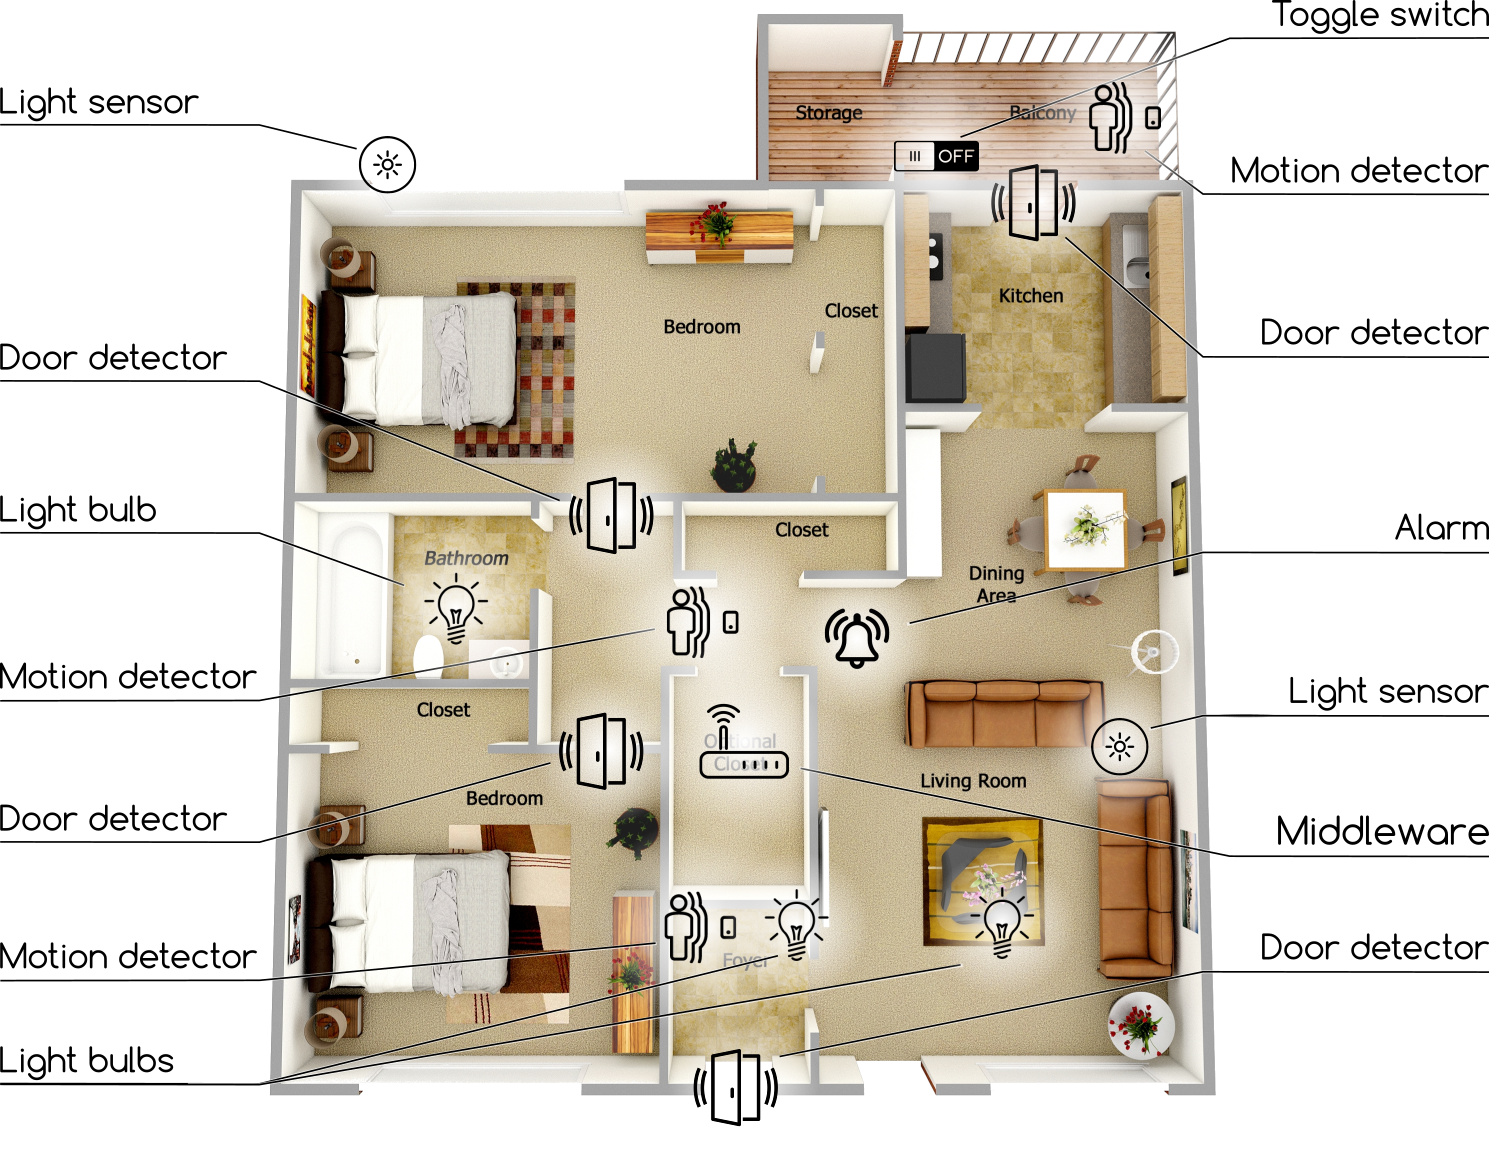
\includegraphics[width=.9\linewidth]{scenario.png}%
	\caption{Hypothetical Alice's \textit{smart-home} configuration of \IOT devices}%
	\label{fig:scenario}%
\end{figure}

Alice is interested in simple scenarios for her comfort and her little boy's security: she wants the entrance lights to automatically switch on to welcome her when she arrives home; 
%she likes her apartment to stay reasonably warm along the year; 
and since her boy often plays in the balcony, or sometimes wakes up at night and walks through the apartment, she needs to ensure he does not fall or injure himself.
Those scenarios seem already possible with the equipment she currently has: we will show how to implement them through a rule-based specification in Section \ref{sec:IoTDSL-BusinessRules}.

%This typical smart home configuration consists of light sensors and bulbs to handle the light in the apartment, motion and door detectors to verify the presence of persons, an alarm in case of emergency and a toggle switch on the balcony. Even if the amount of types of devices is rather limited, we can already highlight a set of features absolutely needed to describe the devices, network configuration and specify its dynamic aspects.


\section{Challenges}
\label{sec:Challenges}

\begin{description}
	\item[Capability Discovery] Providing the ability to drive interconnected devices assumes the capacity of automatically discovering devices' capabilities in a standardised and uniform way. Similar processes happened for other technologies: for example, an \textsc{Usb} device plugged into a computer automatically exposes its nature (e.g., a pointing or video device) and capabilities. This also requires a large ontology that classifies the many dimensions IoT devices are capable of (e.g., \cite{}).
	
	\item[Low-Level Event Reification] Furthermore, the events selected by the device constructors for operating one device could be radically different from what an end-user would expect to drive a particular solution: e.g., a heart rate monitor needs to scan pulsations every millisecond while what interests the user is the rate per minutes. An effective solution for defining high-level customised usage scenarios requires that a mapping between events perceived within a \textsc{Dsl} are bidirectionally mapped to low-level device events, or other artefacts that govern devices' functionalities. Symetrically, the open question of exposing low-level events to users can be useful for some scenarios, but critical in other situations. 
	
	\item[Protocol Interoperability] A domotic solution with heterogeneous devices would often integrate devices from various constructors, thus communicating through multiple communication protocols. In order to make them communicate efficiently, without forcing end-users to stick with one constructor that can dictate costs and restrictions without any control, a powerful \textsc{Dsl} should provide ways for interoperability over multiple communication protocols, without forcing end-users to understand the protocols' intricacies, version evolution, and restrictions.
	
	\item[Reactive Framework for \textsc{Bl}] 
	
	\item[Complex Event Processing (\textsc{Cep})] consists of deriving meaningful conclusions from a stream of events occuring within a system and of responding to them as quickly as possible. 
	%, by tracking and analysing them with various techniques, such as pattern detection, abstraction, filtering, relationship detection, and transformation.
	
	\item[Decentralisation Features] 
	
	\item[Non-Functional Properties] 
\end{description}

\subsection{Components for an \IOT Language}
\label{sec:Motivation-Components}

We argue that a good way of capturing the many variations of scenarios relying on a specific \IOT system deployed at home would consists in offering end users, i.e. home inhabitants like Alice, and technicians in charge of configuring such systems and effectively deploying them, a \DSL that provides at least the following components:

\begin{description}
	\item[Device Description] We need facility to make a precise inventory of the devices used in a specific deployment as well as the high-level capabilities of these devices, described in terms that are immediately understandable by end-users, as opposed to conveying technical details about how those devices precisely operate;
	
	\item[Network Description] A way to capture where each device is located and how it is possible to communicate with it, in order to receive or send data to it;
	
	\item[Dynamics] A way to describe the interactions wished by end-users, \textit{i.e.} how to leverage the functionalities of the devices to effectively realise one or several scenarios that are convenient for the end-users.  
\end{description}

Those components are obviously not sufficient to obtain a fully-fledged solution that becomes adaptable to any situation, but they still represent necessary steps to provide end-users the capacity to manipulate a collection of devices without relying on specific technologies. Defining such \DSLS should encompass a series of facilities dedicated to hide hardware- and protocol-related constraints, and high-level models of devices should somehow be easily \emph{transformable} and \emph{traceable} into concrete infrastructures with simulation and verification possibilities.

